\documentclass[11pt,a4paper]{article}
\usepackage[utf8]{inputenc}
\usepackage{amsmath,amsfonts,amssymb}
\usepackage{graphicx}
\usepackage{geometry}
\geometry{margin=1in}
\usepackage{booktabs}
\usepackage{hyperref}
\usepackage{float}
\usepackage{xcolor}

\definecolor{darkbg}{HTML}{0d121f}
\definecolor{lighttext}{HTML}{e2e8f0}
\definecolor{primary}{HTML}{8b5cf6}
\definecolor{secondary}{HTML}{0dd5c5}

\pagecolor{darkbg}
\color{lighttext}

\hypersetup{
    colorlinks=true,
    linkcolor=secondary,
    urlcolor=secondary
}

\title{\textbf{EE3621: Digital Signal Processing} \\ \Large Lecture 29: DSP for Radar --- Pulse Compression, Doppler Processing \& CFAR \\ \large (III B.Tech EEE)}
\author{Lecture Notes (40-Minute Plan)}
\date{}

\begin{document}

\maketitle

\section{Lecture Plan \& Objectives (40 Minutes Breakdown)}
\begin{itemize}
    \item \textbf{00:00 -- 05:00 (5 mins):} Radar Fundamentals: Range, Doppler, and Resolutions.
    \item \textbf{05:00 -- 12:00 (7 mins):} Matched Filter \& LFM (Chirp): Waveform equations and Pulse Compression.
    \item \textbf{12:00 -- 18:00 (6 mins):} Pulse Compression Implementation: Stretch processing \& FFT.
    \item \textbf{18:00 -- 25:00 (7 mins):} Range-Slow Time Matrix \& Doppler Processing: MTI \& Pulse-Doppler.
    \item \textbf{25:00 -- 30:00 (5 mins):} Constant False Alarm Rate (CFAR) Detection.
    \item \textbf{30:00 -- 35:00 (5 mins):} FMCW Radar \& SAR Basics.
    \item \textbf{35:00 -- 40:00 (5 mins):} Checkpoints \& Review.
\end{itemize}

\noindent\rule{\textwidth}{0.5pt}

\section{Radar Fundamentals}
\subsection{Range Equation}
Radar transmits an electromagnetic pulse and waits for the echo. Let the time-of-flight of the pulse be $\tau$. The round-trip distance is $c\tau$, so the target range $R$ is:
\begin{equation}
R = \frac{c\tau}{2}
\end{equation}

\subsection{Doppler Frequency}
If a target is moving with radial velocity $v$, the round trip distance changes as $2vt$, introducing a phase shift $\phi(t) = - \frac{2\pi (2vt)}{\lambda}$. The Doppler frequency shift is:
\begin{equation}
f_d = -\frac{1}{2\pi} \frac{d\phi}{dt} = \frac{2v}{\lambda}
\end{equation}

\subsection{Resolutions}
The range resolution $\delta R$ and Doppler resolution $\delta v$ are:
\begin{align}
\delta R &= \frac{c}{2B} \\
\delta v &= \frac{\lambda}{2T_{dwell}}
\end{align}

\section{Matched Filter for Radar}

\begin{figure}[H]
    \centering
    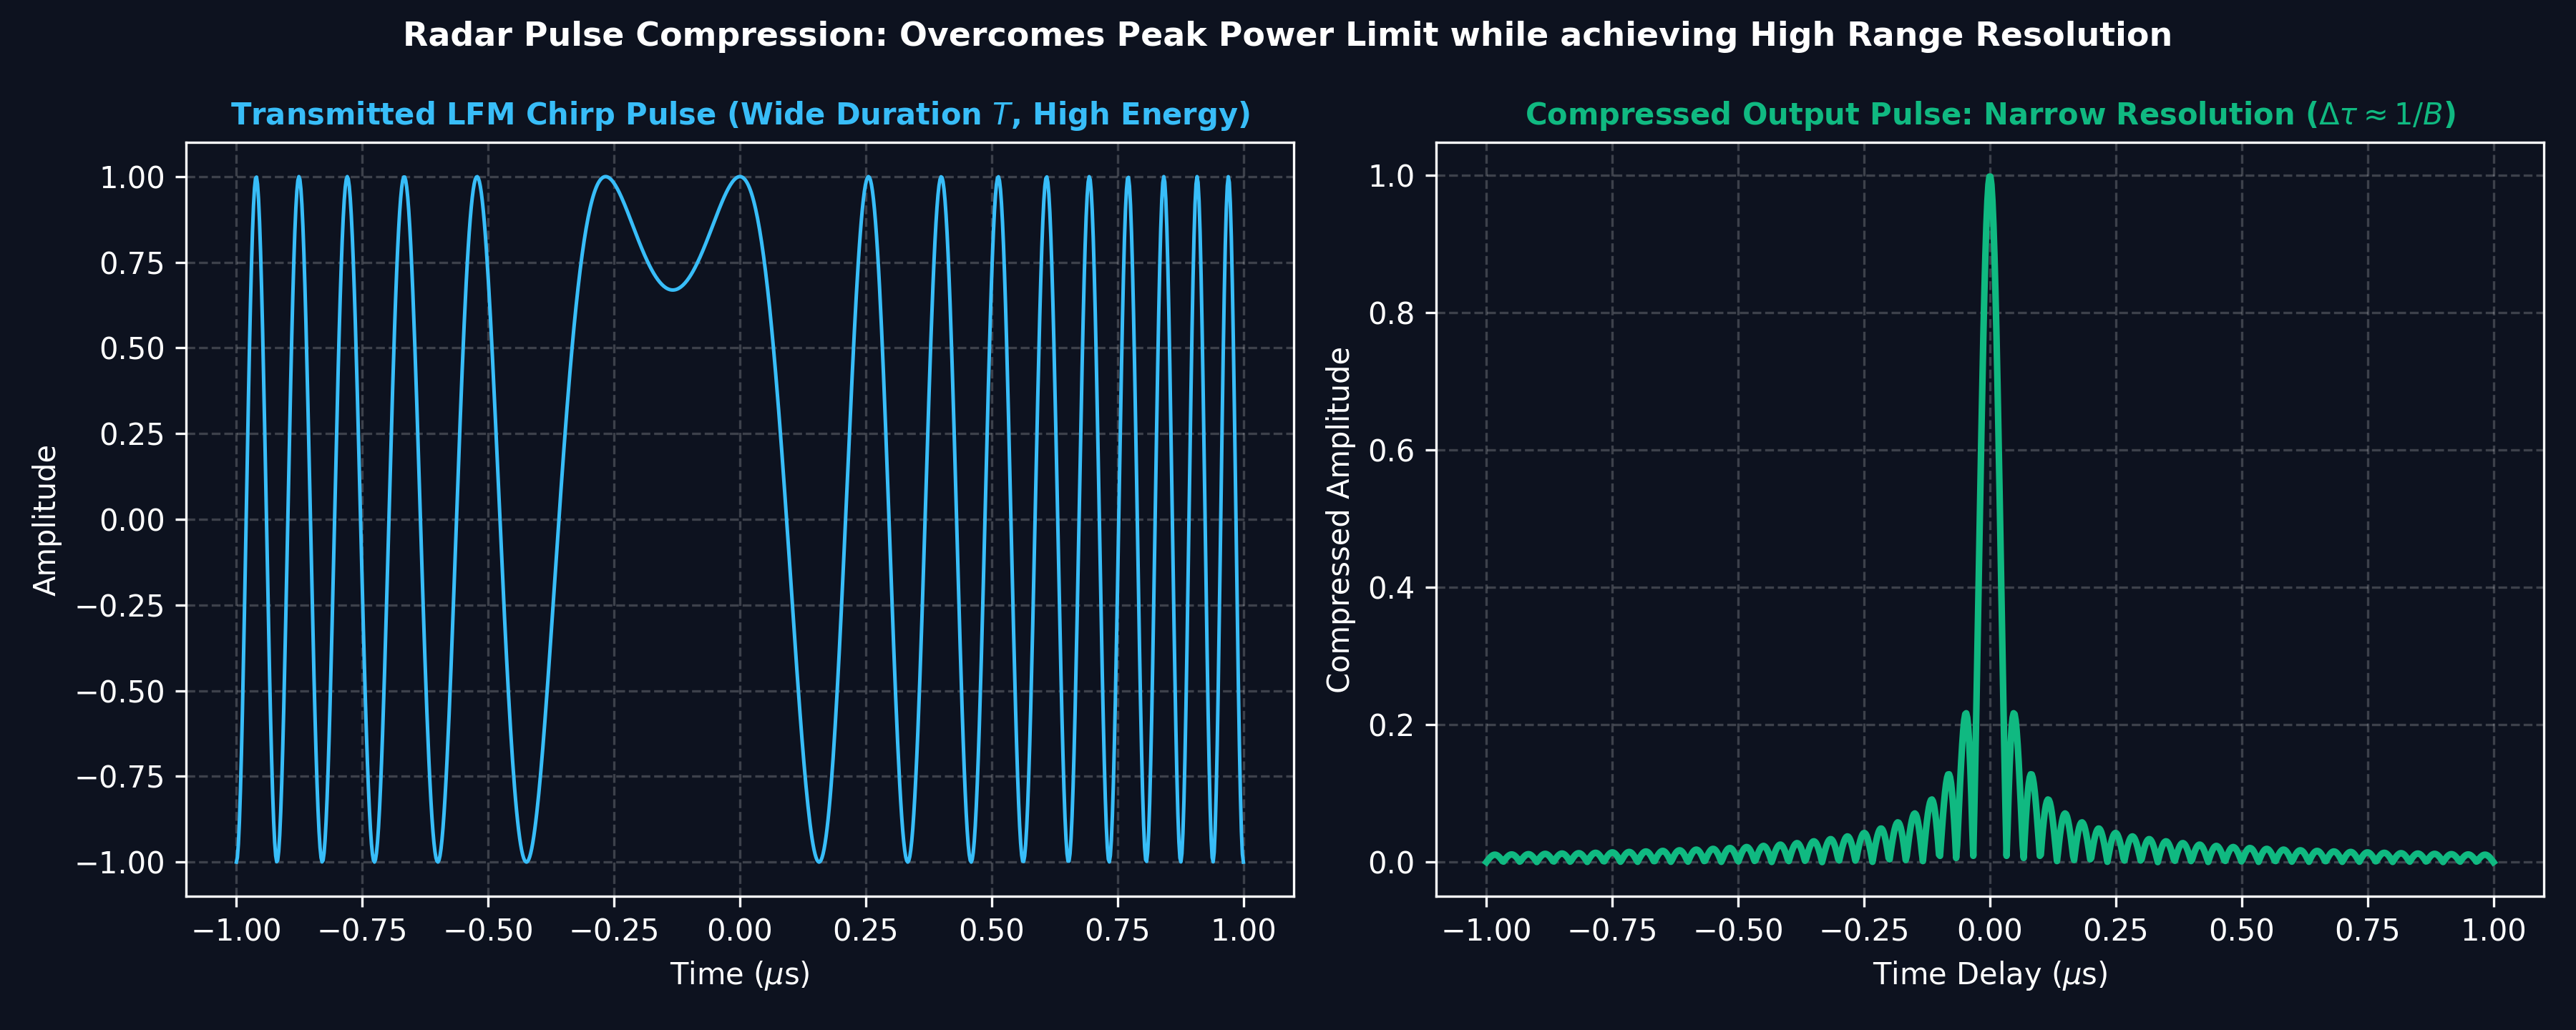
\includegraphics[width=0.85\textwidth]{images/radar_pulse_compression_chirp.png}
    \caption{Radar Linear Frequency Modulation (Chirp) Pulse Compression for High Range Resolution.}
\end{figure}

\begin{figure}[H]
    \centering
    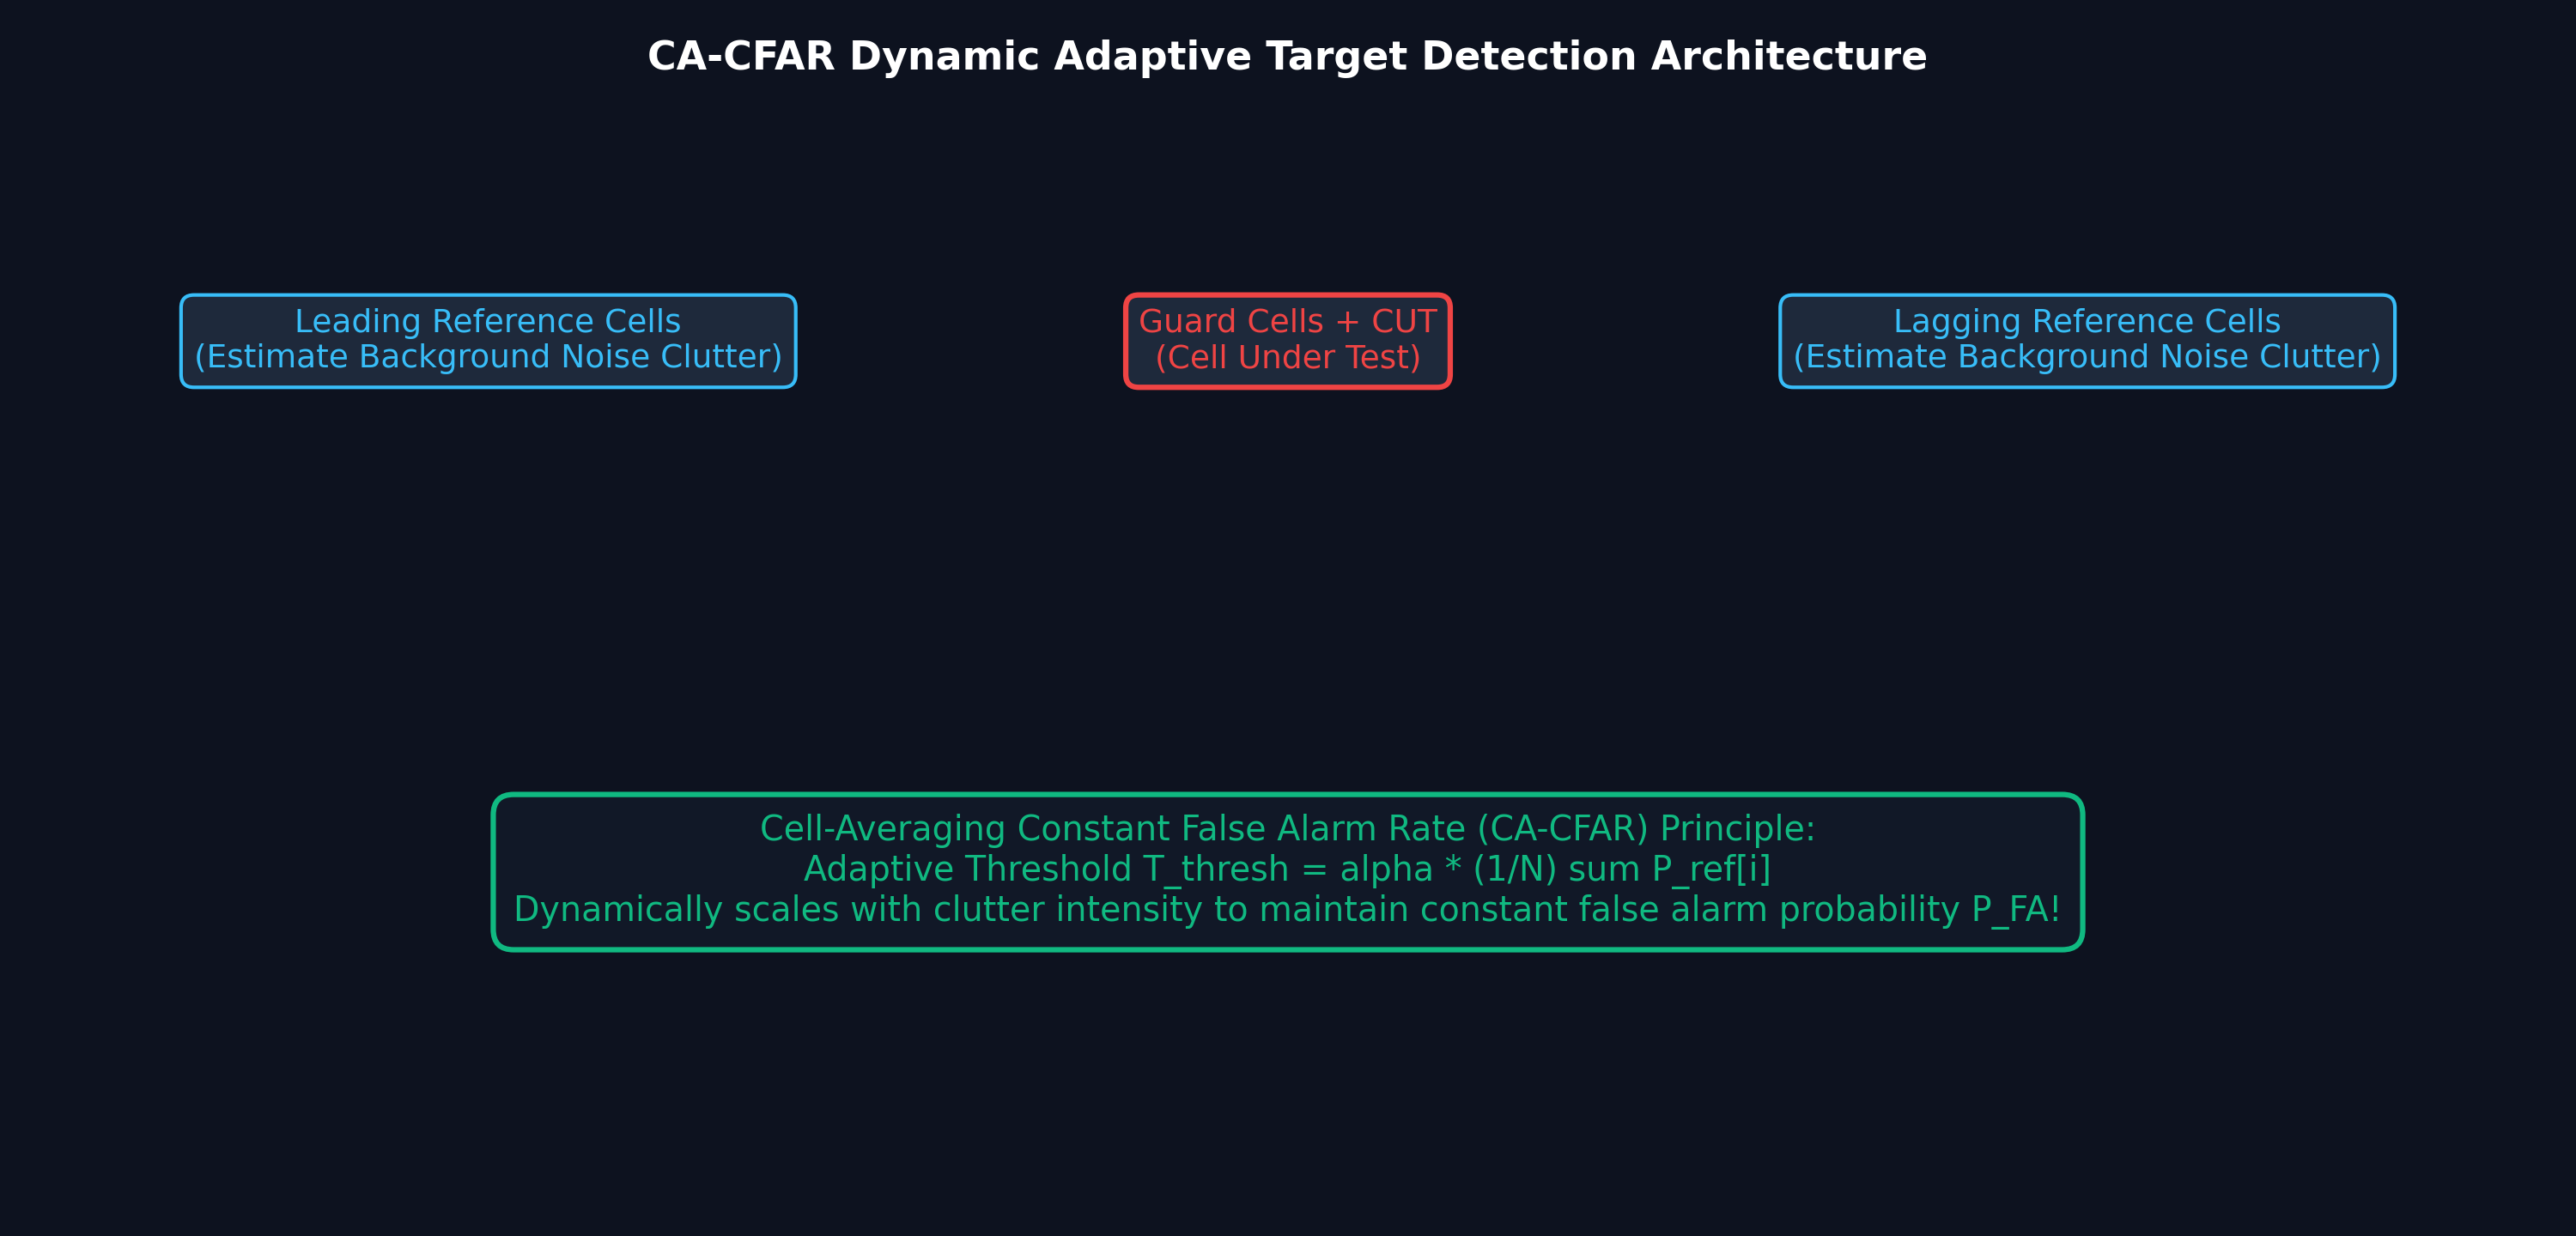
\includegraphics[width=0.85\textwidth]{images/ca_cfar_detection_threshold.png}
    \caption{Cell-Averaging Constant False Alarm Rate (CA-CFAR) Adaptive Threshold Target Detection.}
\end{figure}


\subsection{Linear Frequency Modulated (LFM) Chirp}
The LFM chirp signal is defined as:
\begin{equation}
s(t) = \text{rect}(t/T) e^{j\pi\mu t^2}
\end{equation}
where $\mu = B/T$ is the chirp rate. 

\subsection{Matched Filter Response}
The matched filter impulse response is:
\begin{equation}
h(t) = s^*(-t)
\end{equation}
The output pulse compression is:
\begin{equation}
|R_{ss}(\tau)|^2 = T^2 \text{sinc}^2(\pi B\tau)
\end{equation}
The Time-Bandwidth Product (TBP) represents the compression ratio:
\begin{equation}
\text{TBP} = B \cdot T
\end{equation}

\section{Pulse Compression Implementation}
We use the Frequency Domain for fast processing:
\begin{equation}
Y(f) = R(f)H^*(f) = R(f)S^*(f)
\end{equation}
This is implemented as an FFT-Multiply-IFFT structure. For extreme bandwidths, stretch processing mixes the signal with a reference chirp.

\section{Range Cell Processing}
A radar transmits $N_{chirps}$ pulses. We stack each received pulse into a 2D \textbf{Range-Slow Time Matrix}, where rows are range bins and columns are successive pulses.

\section{Doppler Processing (MTI \& Pulse-Doppler)}
\subsection{Moving Target Indicator (MTI)}
MTI subtracts consecutive pulses to cancel stationary clutter:
\begin{equation}
y(n) = x(n) - x(n-1)
\end{equation}
In designing more complex MTI filters, analog prototype filters can be digitized using the Matched Z-Transform (MZT) (Figure~\ref{fig:mzt}).

Spectral transformations can adapt the MTI notch (Figure~\ref{fig:spectral}).


\subsection{Pulse-Doppler Processing}
A 2D FFT over the Range-Slow Time Matrix produces a \textbf{Range-Doppler Map}, providing both distance and velocity.

\section{Constant False Alarm Rate (CFAR) Detection}
The threshold is $T_{thresh} = T \cdot \bar{P}_{noise}$. For Cell Averaging CFAR (CA-CFAR) with $N$ reference cells and false alarm probability $P_{fa}$, the multiplier is:
\begin{equation}
T = N\left( P_{fa}^{-1/N} - 1 \right)
\end{equation}

\section{FMCW Radar \& SAR Basics}
\subsection{FMCW Radar}
The beat frequency for a stationary target is:
\begin{equation}
f_b = \frac{2R}{c} \frac{B}{T}
\end{equation}

\subsection{SAR Basics}
Synthetic Aperture Radar produces high-resolution images. The azimuth resolution is surprisingly independent of range:
\begin{equation}
\delta a = \frac{D}{2}
\end{equation}

\section{Checkpoint \& Quick Review Questions}
\textbf{Q1:} Calculate range resolution and TBP for $B = 50 \text{ MHz}$ and $T = 20 \mu s$.\\
\textit{Answer:} $\delta R = \frac{c}{2B} = 3 \text{ m}$. $TBP = 50 \times 10^6 \times 20 \times 10^{-6} = 1000$. \\
\\
\textbf{Q2:} Find CFAR threshold $T$ for $N=16$ and $P_{fa} = 10^{-6}$.\\
\textit{Answer:} $T = 16((10^{-6})^{-1/16} - 1) = 16(10^{0.375} - 1) \approx 21.94$.\\
\\
\textbf{Q3:} An FMCW radar with $B = 1 \text{ GHz}$ and $T = 100 \mu s$ has a beat frequency of $150 \text{ kHz}$. Find range $R$.\\
\textit{Answer:} $R = \frac{f_b c T}{2B} = \frac{150 \times 10^3 \times 3 \times 10^8 \times 100 \times 10^{-6}}{2 \times 10^9} = 2.25 \text{ m}$.

\end{document}
